% Section 3 — Approach: the capability-adaptive agent
% Page budget: ~2.5 pages in acmart sigconf two-column (~2200 words).
%
% Source-of-truth verification (no fake info):
%   - 6-layer architecture and 6 controller branches: DOCS/docs8/AGENTIC-SYSTEM-V3.md §4, §8
%   - Skill counts: enumerated against src/agent/skills/ source files 2026-06-16
%       (11 per-window cascade-derived primitives + 4 evidence tools + 1
%       rerank skill = 16 per-window skills; extract_entities_llm is
%       indexing-time only and not counted in the per-window plan)
%   - Failure-mode taxonomy: src/agent/tool_protocol.py FAILURE_* constants
%   - Ring-buffer size 12: src/agent/state/state_layer.py:42
%   - BiEncoder negative sampling: scripts/research-lab/run_biencoder_wol_mode3.py
%       defaults (n_hard_negs=2, n_random_negs=1)
%
% Editorial discipline:
%   - Describe the IDEA, not the implementation primitive. No class names,
%     no Python module paths, no YAML keys. Where a Python class is
%     load-bearing in the architecture, refer to it by its role.
%   - No numbers that are downstream results. Those live in §5-§6.
%   - The cascade-derived skills are presented as DIAGNOSTIC PRIMITIVES
%     the agent draws from, not as a competing system. The cascade is
%     internal-only to this paper.

\section{Approach}
\label{sec:approach}

\subsection{Design philosophy and overview}
\label{sec:approach:overview}

The agent is built around a simple operating principle: \emph{spend on each incident window only what the evidence in that window justifies}. A pre-fault baseline window with no anomalous signal need not invoke a language model; a low-confidence retrieval over an active fault window should. The architecture turns that principle into a per-window decision rather than a deployment-time one, so that the cost-versus-coverage trade-off becomes a property the agent makes case-by-case rather than a knob the operator must set once.

To make this work, six concerns are factored into separate layers, each replaceable without touching the others.

\paragraphhead{(1) An evidence inspector} reads each window's available signals---numeric features, ordered or unordered logs, trace summaries, Kubernetes events, metric snapshots, free-text evidence---and emits a structured \emph{capability set} describing what evidence is present and at what richness.

\paragraphhead{(2) A controller} reads the capability set together with a per-service view of recent monitoring state and emits a \emph{per-window plan}: an ordered list of diagnostic primitives to invoke, each with a per-call budget and an optional gate that the runner consults before executing.

\paragraphhead{(3) A skill registry} holds the diagnostic primitives themselves---retrievers, classifiers, composers, a language-model verifier, a query reformulator, and a small family of on-demand evidence-fetching tools.

\paragraphhead{(4) A runner} walks the plan, evaluates each gate, consults a content-addressed cache, enforces the budget, and writes a per-window execution trace.

\paragraphhead{(5) An on-demand evidence-gathering loop} is the agent's tool-use mechanism: when retrieval consensus is low the runner can fetch additional evidence and re-rank candidates accordingly.

\paragraphhead{(6) A cross-window state layer} keeps a small per-service ring buffer of recent decisions and applies a conservative page-suppression rule that converts repeated alerts on the same incident into one paged ticket.

Every diagnostic invocation is cacheable; every decision is replayable from the trace; every layer is unit-tested in isolation. The remainder of this section walks through each layer, explains the design choices, and notes which mechanisms exist to keep the system honest under measurement.

\subsection{The diagnostic primitives}
\label{sec:approach:primitives}

The skill registry holds sixteen diagnostic primitives the controller can invoke per window---eleven cascade-derived retrieval, verification, and composition primitives, four on-demand evidence-fetching tools, and a re-ranking step that consumes the tools' output. We group them here by per-call cost and the role they typically play in a plan.

\paragraphhead{Cheap path.} Two primitives carry the cheap, every-window cost. The first is a histogram gradient-boosted classifier on a fixed-dimensional vector of pre-computed numeric features summarising the window's logs, traces, metrics, and Kubernetes-state counters (\S\ref{sec:evaluation:datasets} describes the construction). The classifier is small, fits in seconds, requires no standardisation, and outputs a calibrated probability that the window is worth a paged ticket. The second is a fine-tuned dense bi-encoder: a small pretrained Transformer encoder, trained with a contrastive ranking objective so that each (window, gold-ticket) pair dominates other pairs in the batch with two hard negatives mined from sparse retrieval plus one random negative. Retrieval is a cosine product over precomputed memory embeddings, and three similarity-derived features (the top-one cosine, the mean of the top-five cosines, and the count of memory documents above a similarity floor) feed a small logistic regression that converts the retrieval distribution into a triage probability. Together these two primitives form the agent's first line: cheap, fast, and informative enough that on the majority of windows no further work is needed.

\paragraphhead{Escalation retrievers.} Three primitives run only when the cheap path is uncertain. The first is a log-sequence retriever: each log line is independently embedded by a frozen sentence transformer, the resulting sequence of line embeddings is processed by a small transformer encoder with a learned classification token, and the model is trained from scratch on (window-log-sequence, gold-ticket-text) pairs with the same contrastive objective as the bi-encoder. This primitive is weak on average but exceptionally strong on scenario families whose log signature is stereotyped---product-catalog outages, single-pod restarts in healthy replica sets, and slow-recovery windows---because those windows are distinguished by an ordering pattern that bag-of-words representations cannot see.

The second and third are two hybrid sparse-plus-dense retrievers that combine a learned-sparse encoder, the dense bi-encoder, and a structural graph score (described below) into a single ranked list via Reciprocal Rank Fusion~\cite{cormack2009rrf}. The two variants differ only in how query-side entities are extracted at retrieval time: one uses hand-written rules over a canonical vocabulary, the other invokes a language model under a strict JSON schema. The language-model variant is more precise per entity but produces sparser overlap sets; this affects how the controller weights the two variants in different branches.

\paragraphhead{Structural retriever.} A fourth escalation primitive scores past tickets by weighted entity overlap against a small knowledge graph populated once, offline, from a language-model extraction pass over each memory ticket's text. The graph carries one node per memory ticket plus typed nodes for affected services, components, observable symptoms, error classes, root causes, and resolutions, with edges linking each ticket to the entities it mentions (Figure~\ref{fig:kg-vis}). At query time the live window's entities are extracted by the same canonical-vocabulary rule extractor used by one of the hybrid variants, and a parameterised graph query scores each ticket by an additive overlap function that weights error-class matches more highly than service matches, service matches more highly than component matches, and component matches more highly than symptom matches.

\begin{figure*}[t]
  \centering
  \begin{subfigure}[t]{0.55\linewidth}
    \centering
    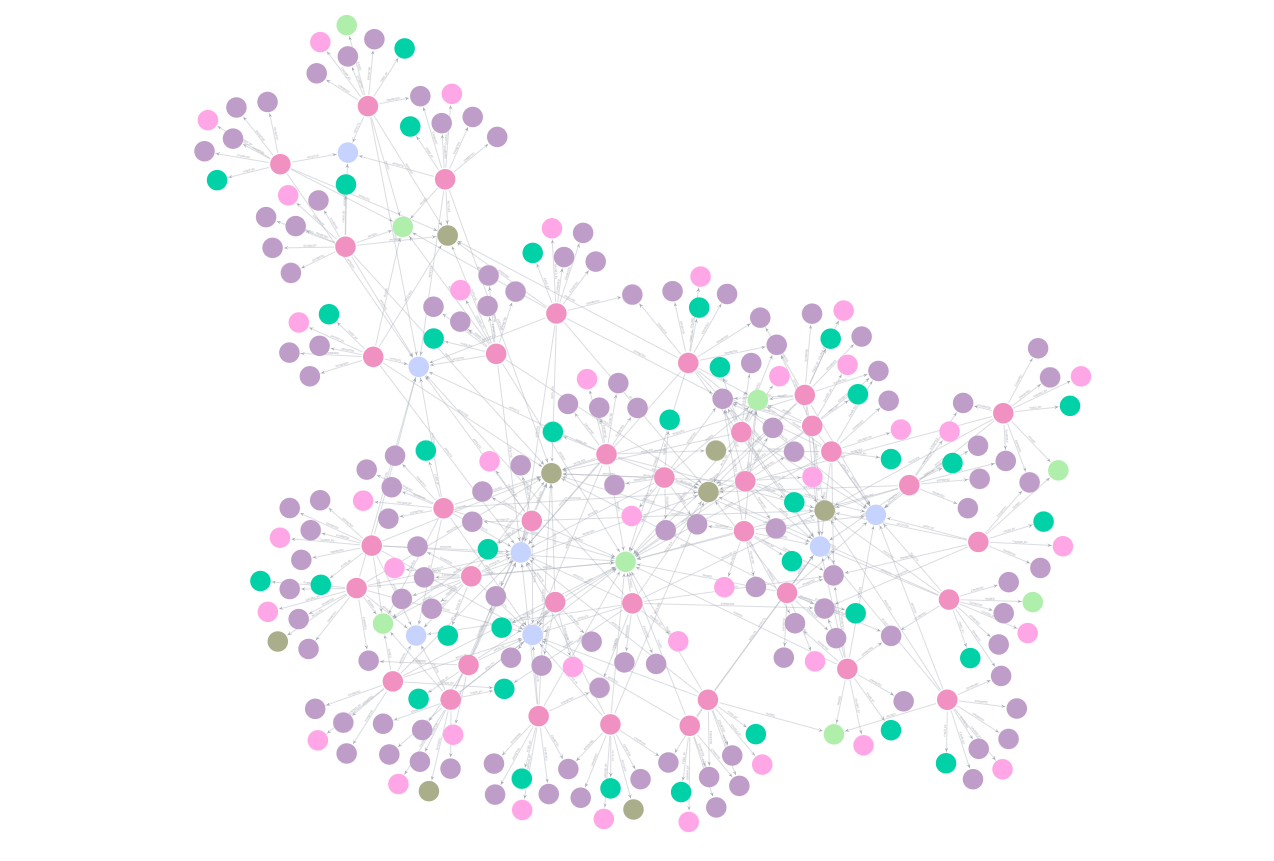
\includegraphics[width=\linewidth]{figures/full-visualisation.png}
    \caption{Whole-graph view. All $347$ incident nodes (pink hubs) plus the typed entity nodes they link to.}
    \label{fig:kg-vis:full}
  \end{subfigure}
  \hfill
  \begin{subfigure}[t]{0.43\linewidth}
    \centering
    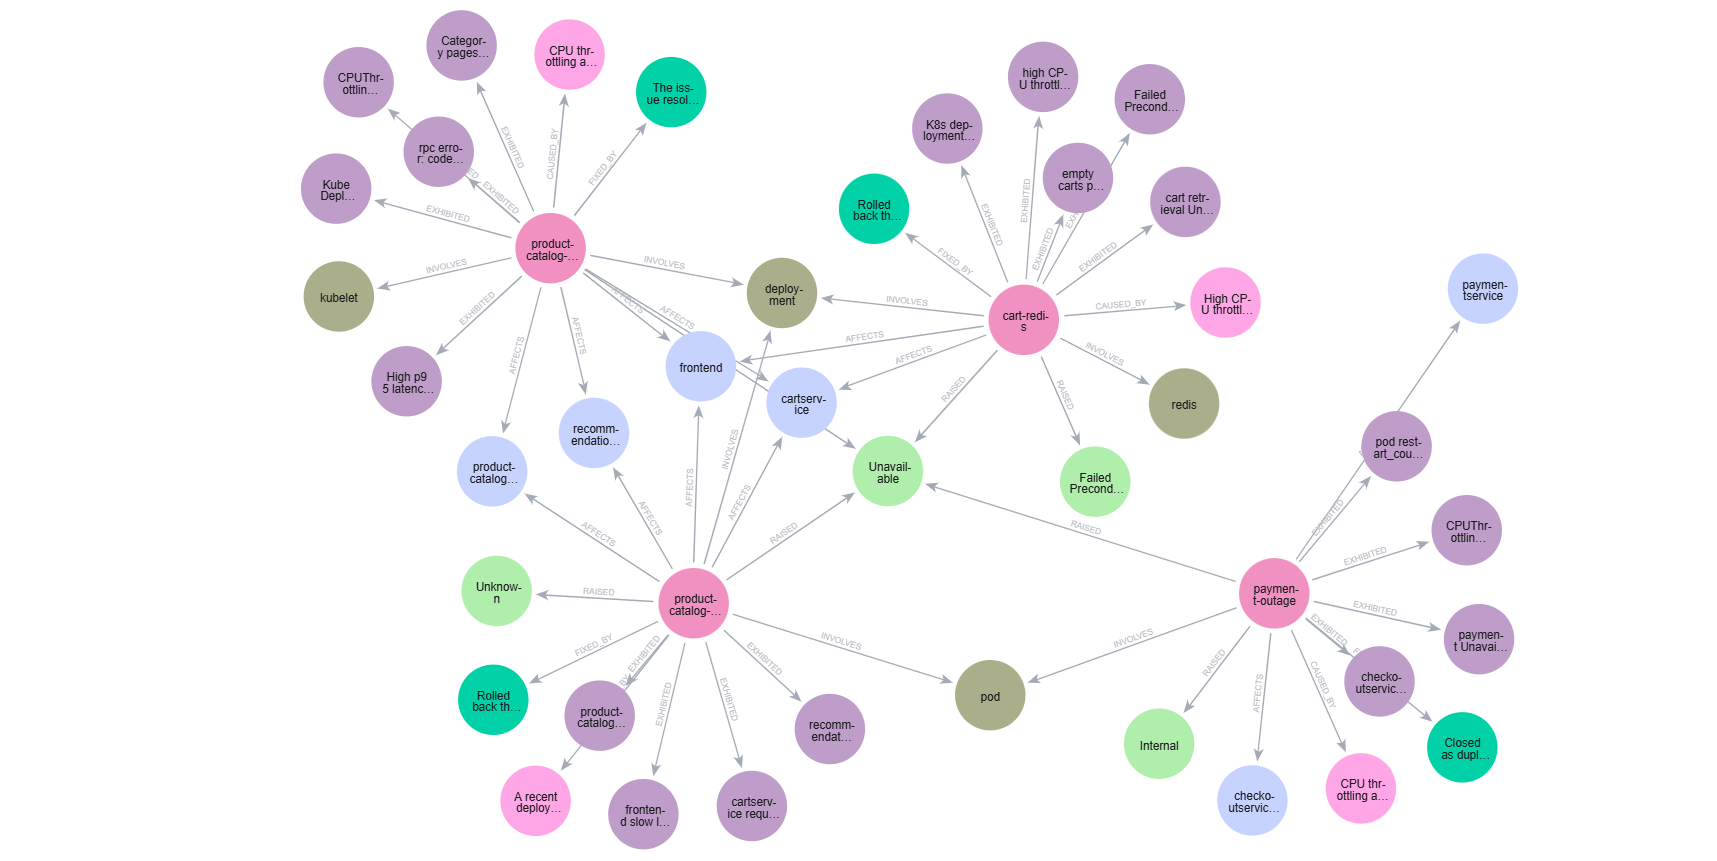
\includegraphics[width=\linewidth]{figures/visualisation2.png}
    \caption{Zoomed view: four incidents and their full one-hop neighbourhoods, showing typed relationships between incidents and entities.}
    \label{fig:kg-vis:zoom}
  \end{subfigure}
  \caption{The memory-side knowledge graph used by the structural retriever and as a sub-retriever inside the hybrid pipelines. One incident node per memory ticket plus typed entity nodes (service, component, error-class, symptom, root-cause, fix). The graph is populated once, offline, from a language-model extraction over each ticket's text; entity overlap between a live window's extracted entities and an incident's connected entities is the retrieval score.}
  \label{fig:kg-vis}
\end{figure*}

\paragraphhead{Language-model verifier.} A primitive that, given the window's evidence text and a small set of candidate tickets, scores each candidate's consistency with an extracted root-cause hypothesis on a calibrated zero-to-one scale and marks each as a worthwhile lead or not. When no candidate clears the consistency threshold the primitive also emits a Boolean novelty flag. The verifier is the only primitive in the registry that performs an explicit comparison between a hypothesised cause and each candidate's recorded cause, and it is the only primitive that emits a novelty signal directly. It is also the most expensive primitive in the registry: a single call typically consumes several thousand prompt tokens.

\paragraphhead{Composition primitives.} Three primitives consume the outputs of the retrievers and the verifier and produce final-form outputs. The retrieval composer takes the dense retriever's three highest-ranked candidates as an anchor pool, re-ranks them by how strongly other retrievers concur, and fills positions two through five via Reciprocal Rank Fusion over the broader retriever set. The triage composer fits a class-balanced logistic stacker over the per-primitive triage scores and emits a single calibrated probability. The novelty composer OR-combines the verifier's novelty flag, a threshold over the maximum retriever confidence, and a learned classifier over coarse window metadata. We use OR rather than weighted combination because the three novelty signals capture qualitatively different forms of evidence and we want any of them to trigger novelty review.

\paragraphhead{Reformulator.} A primitive that, when retrieval consensus is low, edits the query under a bounded action space (drop a token, add a service name, substitute a synonym) and lets the controller re-attempt retrieval. The reformulator is exercised in the trace and its effect is reported in \S\ref{sec:results}.

\paragraphhead{On-demand evidence-gathering tools and reranker.} Four primitives can be invoked when retrieval consensus is low, to fetch additional evidence directly from the raw telemetry the loaders did not stage into the bundle. The \emph{pod-event tool} reads recent Kubernetes warning events for the window's run; the \emph{extended-trace tool} summarises the window's trace dump into a count of distinct services seen and the names of any error spans; the \emph{Prometheus-snapshot tool} extracts restart-delta, CPU and memory peaks, and the count of currently-firing alerts; the \emph{peer-incident tool} retrieves the top-$k$ tickets in the memory corpus that share the window's scenario family, excluding the current incident's own tickets. A \emph{rerank step} consumes the tools' outputs, tokenises each, scores the retrieval composer's top-$k$ candidates by token overlap with each candidate's memory-side text, and emits a re-ranked list. Each tool tags its result with a failure-mode label (success, empty, loop-detected, budget-exhausted, error) so that downstream consumers know to ignore unhelpful tool output (\S\ref{sec:approach:tooluse}).

\paragraphhead{An indexing-time skill.} One further skill, an entity extractor, runs only at memory-corpus construction time: it sweeps each memory ticket's free text once and writes typed entities into the knowledge graph used by the structural retriever and the hybrid retrievers' graph score. Because it never enters a per-window plan, we exclude it from the sixteen runtime primitives counted above.

\subsection{Evidence-driven gating}
\label{sec:approach:gating}

The evidence inspector observes each window and produces a capability set: a frozen collection of presence flags (does this window carry numeric features? ordered logs? trace summary? Kubernetes events? metric snapshots? text evidence? memory text?) together with richness metadata (how many log lines? how many trace spans?). Every primitive in the registry declares the capability flags it requires; the controller can invoke a primitive only when all of its required flags are present. The numeric-feature classifier requires numeric features, so it is automatically dropped on text-only datasets; the language-model verifier requires a verifier-known-helpful flag, so it is structurally skipped on datasets where prior measurement shows it harms retrieval (\S\ref{sec:results}); the log-sequence retriever requires ordered logs, so it is dropped on datasets whose logs are unordered fragments.

The inspector exposes two further mechanisms used for evaluation. First, a capability \emph{mask} drops named flags from the inspector's output before the controller sees them, which lets us run the agent on a dataset under counterfactual capability conditions (\S\ref{sec:results}, RQ-C4). Second, a verifier-calibration table lists which datasets the language-model verifier is known to be helpful on, which it is known to be harmful on, and a default policy for unrecognised datasets. Because the verifier's required flag is unset for harmful datasets, the system structurally refuses to invoke it on those datasets, regardless of any runtime decision a controller might attempt. This kind of structural refusal---built into the capability layer rather than asserted at runtime---is the discipline that makes our cross-dataset transfer claims auditable.

\subsection{The per-window plan}
\label{sec:approach:plan}

The controller emits one of six branches depending on the window's type and the per-service recent state. The plan is the canonical artifact: it is serialisable, replayable, and inspectable, and every downstream measurement in \S\ref{sec:results} reads from it.

\paragraphhead{State-suppression branch.} When the per-service state layer reports a recent ticket-worthy decision on the same scenario family with no recovery in between, the controller emits a minimal plan that runs only the triage composer using cached upstream outputs. This branch is the cheapest path through the system and is the only one that touches the cross-window state.

\paragraphhead{Pre-fault baseline branch.} When the window's type is a baseline captured before any fault, the controller emits a plan that runs the numeric-feature classifier, the triage composer, and the novelty composer only. Retrievers are skipped because pre-fault baselines are novel by construction.

\paragraphhead{Recovery and observation branches.} When the window's type indicates an active recovery or a non-fault observation period, the controller emits a cheap-path plan that runs the numeric-feature classifier plus the dense retriever plus the composers. Expensive retrievers are skipped: prior measurement (\S\ref{sec:results}) shows that no retriever beyond the dense bi-encoder moves rank-one retrieval on this class of window.

\paragraphhead{Active-fault branch.} The most invocation-rich branch. The plan begins with the cheap path (numeric-feature classifier and dense retriever), then gates each escalation primitive on a runtime check of cheap-path confidence: if the numeric classifier exceeds a confidence threshold and the dense retriever's top-one matches one other voter, the gates close and expensive retrievers are skipped. If the cheap path is uncertain, the gates open and the log-sequence retriever, both hybrid retrievers, and the structural retriever fire in parallel. The retrieval composer then runs over whatever subset actually fired. A second gate, on the retrieval composer's confidence, opens the reformulator and the four on-demand evidence-gathering tools plus the reranker. The triage composer, the language-model verifier (if known-helpful), and the novelty composer run unconditionally at the end of the branch.

\paragraphhead{Default branch.} A fallback that emits the same plan as the active-fault branch, used when the window's type is missing or unrecognised. In practice this branch is rarely emitted on telemetry datasets.

The cheap-first / escalate-on-uncertainty pattern is what produces the cost savings reported in \S\ref{sec:results}. The threshold above which the cheap path is considered confident is a single tunable parameter; we report the sensitivity of the cost-quality trade-off to this parameter in \S\ref{sec:results:pareto}.

\subsection{The on-demand evidence-gathering loop}
\label{sec:approach:tooluse}

The active-fault branch optionally invokes a small loop of evidence-gathering tools when the retrieval composer's top-one confidence is below a configurable floor. The loop is conceptually similar to existing tool-using language-model agents~\cite{yao2023react,schick2023toolformer} but is more conservative in two ways. First, each tool is a deterministic data-lake read rather than a free-form action emitted by a language model. Second, the policy that decides which tools to call is the controller's rule-based branch logic rather than an end-to-end learned policy. This design tradeoff is deliberate: a fixed action space lets us measure the contribution of each tool individually in \S\ref{sec:results} without confounding the measurement with policy learning, and an LLM-emitted-action variant fits cleanly on top of the same protocol as future work.

Each tool, when invoked, returns a structured payload together with a failure-mode tag. We track five failure modes: \emph{hallucinated tool name} (the controller asks for a tool that is not registered---this cannot happen with our rule-based controller but is logged as a defence for a future learned policy); \emph{empty result} (the data lake returned no usable signal, for example because the requested run has no Kubernetes events recorded for that window); \emph{looping repeated call} (the controller has asked for the same tool with the same arguments three times in the same window); \emph{budget exhausted} (the per-window tool-call cap has been hit); and \emph{tool error} (the data-lake read raised an exception). The five-mode taxonomy is reported per-tool per-dataset in \S\ref{sec:results} and is the agent's reviewer-defence against the standard ``what about failure modes?'' question.

The reranker that consumes the tools' output is intentionally simple: it tokenises each tool result, computes the count of tokens shared with each candidate's memory-side text, sorts top-$k$ by overlap with the original retrieval rank as tiebreaker, and emits a new ranked list. We intentionally avoid a learned reranker here: any positive contribution of the loop has to come from the tools' \emph{content}, not from a separately-tuned scoring head.

\subsection{Cross-window state and page suppression}
\label{sec:approach:state}

The state layer keeps a per-service ring buffer of recent decisions (the last twelve windows by default). Each entry records the window's timestamp, the resulting triage decision, the top-ranked past ticket, the predicted novelty flag, and the incident identifier if any. The buffer is read by the controller at plan time (the state-suppression branch consults it) and written by the runner at decision time.

The page-suppression rule is conservative by design. A window's decision is downgraded from \emph{ticket-worthy} to \emph{borderline} and attached to the existing incident only when three conditions all hold: the same top-one past ticket has been emitted on each of the last three contiguous windows for this service, the scenario family has not changed across those windows, and no recovery window has intervened. The same-family check is the load-bearing protection against suppressing a legitimately new incident on the same service. The operational metric, pages per incident, is reported per-dataset in \S\ref{sec:results}.

\subsection{The runner and replayable traces}
\label{sec:approach:runner}

The runner executes a plan one invocation at a time. For each invocation it (i) evaluates the gate, skipping if it returns false; (ii) consults a content-addressed cache keyed on the primitive's identifier and version together with a hash of the window and memory inputs; (iii) checks the remaining per-window budget; (iv) calls the primitive; and (v) writes a trace event recording the primitive's name and version, its output, its actual cost, and a snapshot of the remaining budget.

The cache is on-disk and survives across runs; an ablation that disables one primitive does not re-run any of the others, which is how the per-primitive analyses in \S\ref{sec:results} can be produced cheaply. The budget bounds the total wall time, language-model tokens, and dollar-equivalent cost per window; an exhaustion event is logged and the rest of the plan is aborted gracefully, with the agent surfacing a \emph{needs-review} decision rather than a guess.

The trace is the system's contract with the user. Every decision can be reconstructed from its trace alone: which branch the controller chose, which gates fired, which primitives executed (versus skipped via gate or cache), what each primitive returned, what the cumulative cost was, and what the final decision looked like. Traces are written one JSON file per window under a configurable trace root; they are how every ablation in \S\ref{sec:results} is audited, and they are what a future learned controller would train on.

\subsection{Extensibility}
\label{sec:approach:extensibility}

The layered design is what allows extension to be a local edit rather than an architectural change. Adding a new diagnostic primitive requires implementing the uniform skill interface (declaring the required capability flags, the per-call cost class, the cache key shape, and the invoke method), registering the new class in the skill registry, and referencing it by name in the controller's plan template. No other layer changes. Adding a new evidence modality is a matter of adding a new capability flag, populating it in the evidence inspector when the modality is present, and updating any existing primitive that wants to consume it. Adding a new dataset is a matter of defining a dataset profile that lists the available primitives, the per-skill predictions location, the data-lake root for raw telemetry, and the verifier-calibration policy; the shared harness builder consumes the profile and produces a fully configured agent without further code changes. Adding a new tool to the on-demand loop is a matter of subclassing the evidence-request interface, implementing the data-lake read, registering the new class, and adding the new tool's name to the controller's active-fault branch tool list; the five-mode failure taxonomy applies automatically.

These extension points are not aspirational. They are the same edits used to bring up the second and third datasets in \S\ref{sec:cross-app} and to perform every ablation in \S\ref{sec:results}: every cross-dataset replication in this paper is a profile switch, and every ablation is a local edit. That is what makes the empirical claims that follow stable under measurement.
